
\section{Αριχτεκτονική IRIS (2006) ΗΠΑ}

% ------------------------------------------------------------------------------------------
% ARCHITECTURE OF AN INTEGRATED ROUTER INTERCONNECTED SPECTRALLY
% ------------------------------------------------------------------------------------------

Συνδυάζοντας την εξισορρόπηση φορτίου με τη μεταγωγή μήκους κύματος, η
αρχιτεκτονική IRIS μπορεί να χρησιμοποιήσει χιλιάδες μήκη κύματος και
να παράσχει terabits δυναμικότητας. Η αρχιτεκτονική IRIS χρησιμοποιεί
εξισορρόπηση φορτίου για να εξαλείψει την ανάγκη για κεντρικό
προγραμματισμό, και μεταγωγή μήκους κύματος επιτρέποντας $N^2$
διαύλους σε έναν space switch διακόπτη N × N. Xρησιμοποιεί τεχνικές
εξισορρόπησης φορτίου για την αντιμετώπιση της πολυπλοκότητας του
προγραμματισμού συστήματος των διακοπτών και της προβληματικής χρήσης
δομών τύπου RAM για τη συγκέντρωση των εισερχομένων πακέτων στις
εισόδους. Πρακτικά χρησιμοποιούνται τρία επίπεδα συνδέσεων. Τα
εισερχόμενα πακέτα των N εισόδων, διαμοιράζονται μέσω ενός space
switch με τυχαίο τρόπο σε Ν δομές μνήμης στο μεσαίο επίπεδο. Κάθε
μνήμη του μεσαίου επιπέδου διατηρεί Ν εικονικές ουρές εξόδου, μια για
κάθε θύρα εξόδου, παρόμοια με έναν input-buffered switch. Τα πακέτα
τοποθετούνται στις μνήμες με βάση τον τελικό προορισμό τους. Ένας
space switch στο τρίτο στάδιο δέχεται τα πακέτα αδειάζοντας τις μνήμες
του μεσαίου επιπέδου και τα δρομολογεί στους τελικούς προορισμούς
τους.

\begin{figure}[h]
  \centering
  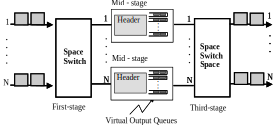
\includegraphics[width=.7\linewidth]{iris.pdf}
  \caption{Η αρχιτεκτονική IRIS}
  \label{fig:iris}
\end{figure}

H έννοια της εξισορρόπησης φορτίου προσφέρει τρία βασικά πλεονεκτήματα
που είναι ιδιαίτερα σημαντικά για τον οπτικό δρομολογητή. Κατ 'αρχάς,
εξαλείφει τον προγραμματισμό και ακόμη μπορεί να εγγυηθεί 100\%
ρυθμαπόδοση, παρέχοντας μια στρατηγική ώστε η κατανομή της κυκλοφορίας
να γίνει ομοιόμορφη και γνωστή, ανεξάρτητα από την πρότερη κατανομή
της κυκλοφορίας. Έτσι οι αλγόριθμοι δυναμικού προγραμματισμού
αντικαθιστούνται από στατικούς, μειώνοντας την
πολυπλοκότητα. Δεύτερον, επιτρέπει τον σχεδιασμό απλών δομών ενταμιευτών
βασισμένων σε delay lines. Τρίτον, ορίζει μια non-blocking
αρχιτεκτονική που θα μπορούσε να βασίζεται σε blocking space switches,
επιτρέποντας έτσι τη δυνατότητα κλιμάκωσης.

Η δυνατότητα επεκτασιμότητας της αρχιτεκτονικής IRIS στηρίζεται
σημαντικά στο γεγονός ότι οι διασυνδέσεις του πρώτου και του τρίτου
επιπέδου δεν πρέπει να είναι απαραίτητα non-blocking. Αυτό μπορεί να
επιτευχθεί επιλέγοντας μόνο N permutations συνδέσεων, όπου σε κάθε μία
από αυτές τις μεταθέσεις μια δεδομένη θύρα εισόδου μπορεί να μεταδώσει
ένα πακέτο σε μια διαφορετική θύρα εξόδου. Ακόμη και αν ένας διακόπτης
επιτρέπει μόνο αυτές τις N μεταθέσεις και εμποδίζει άλλες μεταθέσεις,
μπορεί να χρησιμοποιηθεί σε ένα σύστημα ισορρόπησης φορτίου.  Αυτή η
ιδιότητα μας επιτρέπει να χρησιμοποιούμε scalable blocking wavelength
cross-connects, για να χτίσουμε ένα non-blocking σύστημα. Οπότε,
χρησιμοποιώντας πακέτα δεδομένων 40 Gb / s και 80 × 80 AWGs (Arrayed
Waveguide Gratings), η αρχιτεκτονική αυτή μπορεί να κλιμακωθεί σε $802
\times 40 Gbps = 256 Tbps$.

%%% Local Variables:
%%% mode: latex
%%% TeX-master: "main"
%%% TeX-engine: xetex
%%% End:
